\documentclass[a4paper,12pt]{article}
\title{COMP9444 Neural Networks}

\usepackage{amscd}
\usepackage{amsmath}
\usepackage{amsfonts}
\usepackage{amssymb}
\usepackage{amsthm}
\usepackage[english]{babel}
\usepackage{bm}
\usepackage{color}
\usepackage{dsfont}
\usepackage{epsfig}
\usepackage{enumitem}
\usepackage{esint}
\usepackage{fancyhdr}
\usepackage{fancyvrb}
\usepackage{float}
\usepackage[T1]{fontenc}
\usepackage{geometry}
\usepackage{graphicx}
\usepackage[utf8]{inputenc}
\usepackage{pifont}
\usepackage{latexsym}
\usepackage{lscape}
\usepackage[utf8]{luainputenc} 
\usepackage{mathtools}
\usepackage{multirow}
\usepackage{natbib}
\usepackage{spverbatim}
\usepackage{stackrel}
\usepackage[nottoc]{tocbibind}
\usepackage{units}
\usepackage[svgnames]{xcolor}

\geometry{verbose, margin=1.8cm}
\pagestyle{fancy}

\rhead{Melinda Mortimer (z5016924)}
\lhead{COMP9444 Assignment 2}
\setlength{\headheight}{15pt}

\makeatletter
%%%%%%%%%%%%%%%%%%%%%%%%%%%%%% User specified LaTeX commands.
\date{}

\makeatother

\usepackage{babel}

\newcommand\numberthis{\addtocounter{equation}{1}\tag{\theequation}}
\newcommand{\code}{\texttt}

\begin{document}

\subsection*{Final Model Structure}

\begin{figure}[h]
\begin{center}
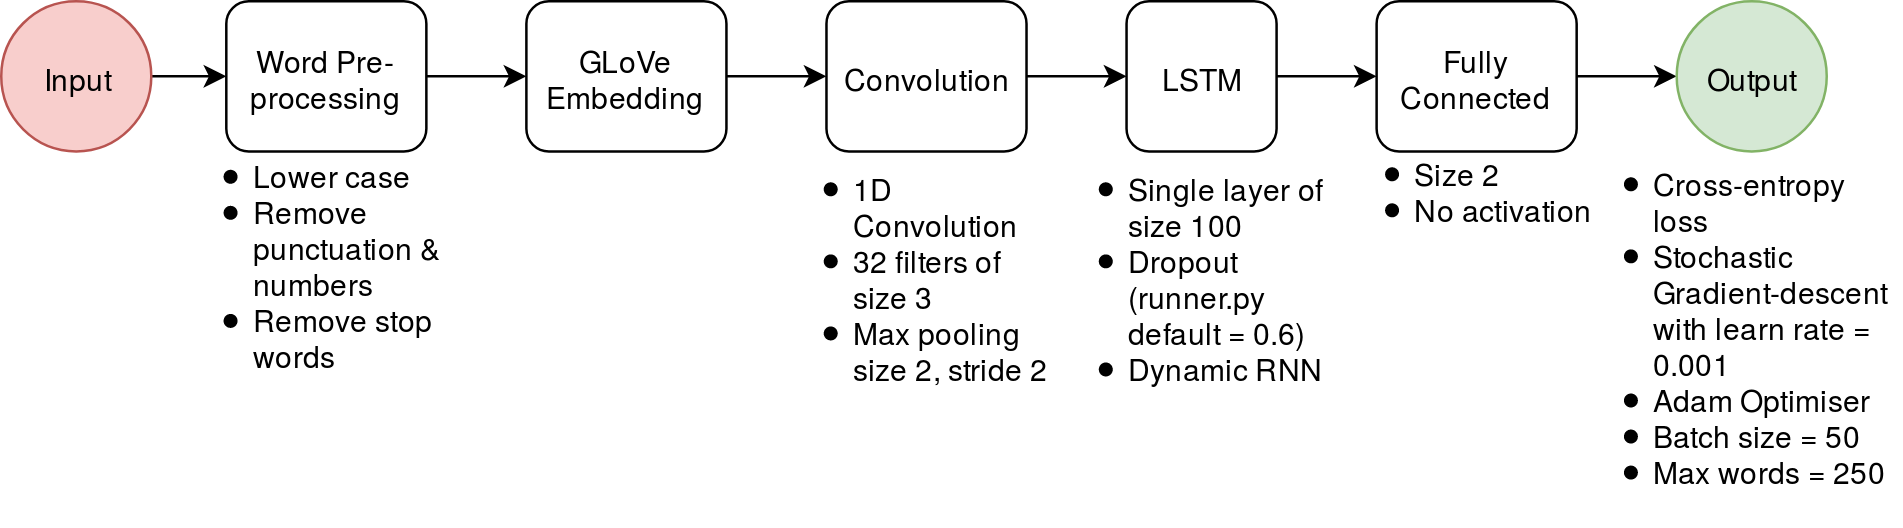
\includegraphics[width=\linewidth]{diagram.png}
\end{center}
\end{figure}

Input sentences were converted into lower case letters. Punctuation and numbers were removed so that only words remain. Stop words were removed to ensure a higher proportion of usable words. GLoVe embedding converts these words into 50-dimensional word vectors.

Initial model attempts were made using a LSTM layer and 1 fully connected layer. In these initial models, experiments with \code{BATCH\_SIZE} and \code{MAX\_WORDS\_IN\_REVIEW} found that smaller batch sizes sped up training time, and a higher number of words improved model accuracy faster. Final values were set to \begin{verbatim}
BATCH_SIZE = 50
MAX_WORDS_IN_REVIEW = 250
\end{verbatim}

A \textit{1D convolution layer} was added to gain context from surrounding words. This layer includes 32 convolution filters, each of size 3. These filters are numerous enough to pick up a large number of features, without overfitting the data. The small filter size ensures that the layer only convolves around nearby words and does not lose context by considering words that are further away. \textit{Max pooling} with size 2 and stride 2 is used to downsample the data, with only a small size to constrict the loss of information.

A \textit{LSTM layer} was included so that the architecture can exhibit a memory of previous cycles. This layer was of size 100, which allowed for enough features to be learned without overfitting. A dropout layer was added to the LSTM as a regularisation technique, helping to avoid overfitting. Dropout rate is a placeholder variable, with the default set to 0.6 in \code{runner.py}. The layer was specified as a dynamic RNN to improve graph creation time and allow for variable size batches if need be.

A \textit{fully connected layer} of size 2 was added to consolidate the features and structure the output. For simplicity, no activation function was included. Softmax activation could have been used instead to output a probability distribution.

\textit{Cross-entropy loss} was used as the expected outputs take on the form of a 0/1 flag. The learning rate for gradient descent was set to 0.001 to ensure quick convergence without overshooting the minimum loss. The Adam Optimiser was chosen so that the learning rates are not necessarily constant across all trained variables.

\textit{Early stopping} was used to avoid overfitting. The model was saved every 1000 steps, and chosen to maximise the validation set. This occurred at step 9000, with a validation accuracy of 84.6\%.




\end{document}
